%!TEX root=../../root.tex
\section{Lezione 20}

\subsection{Complessità di Spazio}

Sia $M$ una macchina di Turing deterministica che si arresta su tutti gli input. La \emph{complessità di spazio} di $M$ è la funzione 
\begin{gather*}
	f:\mathbb{N} \to \mathbb{N}\\
	f(n) = max\{ \text{numero di celle del nastro che } M \text{ scandisce su ogni input di lunghezza } n \}
\end{gather*}
Se $M$ è una macchina di Turing non deterministica in cui tutte le diramazioni si arrestano su tutti gli input, definiamo la sua complessità di spazio \emph{f(n)} come il massimo numero di celle del nastro che \emph{M} scandisce su qualsiasi diramazione della sua computazione per ogni input di lunghezza \emph{n}.

\subsection{Teorema di Savitch}
\newtheorem*{thm}{Teorema}
\begin{thm} 
Se $T \in NTM$ ha complessità di spazio $S_{T}(n)\geq n$, allora $\exists$ $T' \in TM$ equivalente avente complessità di spazio $S_{T'}(n)=O(S^{2}_{T}(n))$. \\
\end{thm}
\begin{proof}[Dimostrazione]
Il teorema si dimostra esibendo una $TM$ deterministica che simula la $NTM$ data in input, che ha complessità di spazio $S_{T}(n)$, usando spazio $O(S^{2}_{T}(n))$.

L'approccio utilizzato per simulare una $NTM$ con una $TM$ deterministica che conosciamo richiede tempo e spazio esponenziali, quindi si usa un approccio differente. Si consideri il problema più generale del \emph{reach}, la cui formulazione è la seguente:

Date due configurazioni $c, c'$ della $NTM$, determinare se essa può transitare da  $c \  \text{a} \ c'$ in al più $t$ passi. Vediamo una implementazione ricorsiva di tale algoritmo.
\paragraph{CANYIELD}
\begin{description}
	\item \textit{input}: \emph{(c,c',t)}
	\item \textit{output}: 1 se $c \Rightarrow^{\star} c'$ in al più \emph{t} passi, 0 altrimenti
	\item \textit{descrizione}:
	\begin{enumerate}[label*=\arabic*.]
		\item Se $t = 0$:
		\begin{enumerate}[label*=\arabic*.]
			\item Se $c = c'$, allora ritorna 1 
			\item Altrimenti ritorna 0 
		\end{enumerate}
		\item Se $t=1$:
			\begin{enumerate}[label*=\arabic*.]
				\item Se $c \Rightarrow c'$, allora ritorna 1
				\item Altrimenti ritorna 0
			\end{enumerate}
		\item $\forall \ c'' \ \text{di} \ T$
			\begin{enumerate}[label*=\arabic*.]
				\item Ritorna \emph{CANYIELD($c$,$c''$,$\frac{t}{2}$)} $\land$ \emph{CANYIELD($c''$,$c'$,$\frac{t}{2}$)}
			\end{enumerate}
	\end{enumerate}
\end{description}
Risolvere tale problema con input ($c_i,c_f,S_T(n)$), dove $c_i$, $c_f$ e $S_T(n)$ sono rispettivamente la configurazione iniziale $(q_0x)$, la configurazione finale $(q_aB)$ e il numero massimo di passi che la $NTM$ può effettuare, equivale a stabilire se la macchina $T$ accetti o no l'input $x$. \\
Notare che esistono diverse possibili configurazioni finali ma per evitare di dover chiamare l'algoritmo per ogni configurazione accettante applichiamo una modifica alla $NTM$ in modo che l'unica configurazione di accettazione sia proprio $q_aB$, ossia quella in cui il nastro è vuoto e la la testina è all'inizio del nastro.
\begin{figure}[H]
    \centering
    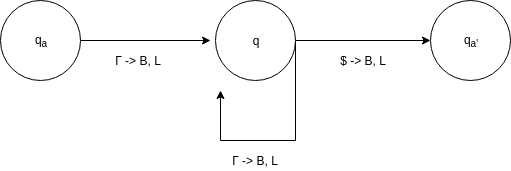
\includegraphics[scale=0.6]{modifica}
\end{figure}

Per capire quanto spazio richiede l'algoritmo analizziamo lo stack delle chiamate ricorsive. Ciascun livello della ricorsione usa spazio \emph{$O(S_{T}(n))$} per memorizzare una configurazione. La profondità della ricorsione è \emph{log t}, dove \emph{t} è il tempo massimo che la NTM può usare su ogni diramazione e che per semplicità assumiamo essere una potenza di 2. Quindi una volta che la ricorsione raggiunge il caso base nello stack delle chiamate ci saranno $O(lg \ t)$ chiamate, ognuna delle quali avrà memorizzato due configurazioni e il valore di t occupando uno spazio di $O(S_T(n)) + O(lg \ t)$.

 Nel nostro caso ci interessa $t=2^{O(S_{T}(n))}$, poiché esso è il tempo che la $TM$ impiega a simulare la $NTM$; quindi $log \ t = O(S_{T}(n))$. Pertanto la simulazione deterministica usa spazio $O(S^2_{T}(n))$.\\
Dobbiamo ora dare la descrizione della macchina deterministica $T'$ equivalente a $T$.

\newpage
$T'$:
\begin{description}
	\item \textit{input: x}  
	\item \textit{descrizione:}
	\begin{enumerate}[label*=\arabic*.]
		\item Esegue \emph{CANYIELD} su ($c_i,c_a,2^{O(S_T(n))}$)
		\begin{enumerate}[label*=\arabic*.]
			\item Se \emph{CANYIELD} ritorna 1, accetta
			\item altrimenti rifiuta
		\end{enumerate}
	\end{enumerate}
\end{description}
L'algoritmo richiede tuttavia in input il parametro \emph{t} che nel nostro caso è $2^{O(S_T(n))}$. Non sapendo $S_T(n)$ dobbiamo sfruttare il fatto che $2^{O(S_T(n))} = 2^{k\cdot S_T(n)}$, $k$ dipende solo da $|\Gamma|$ e $|Q|$ ed è quindi nota, invece per trovare $S_T(n)$  dobbiamo provare tutti i possibili valori $i = 0,1,\dots$ finché non si ottiene l'$S_T(n)$ cercato.

Per far in modo che l'algoritmo si fermi sempre bisogna inoltre controllare ad ogni iterazione che vi sia una configurazione raggiungibile a distanza $i+1$.
\end{proof}

\subsection{PSPACE e NPSPACE}
Per definire le classi $PSPACE$ e $NPSPACE$, ci serviamo di altri due linguaggi ovvero $SPACE$ e $NSPACE$:

$$NSPACE(n^k) = \{ L \mid L \in NTM \land L(T)=L \land S_T(n)=O(n^k) \}$$

$$NPSPACE = \bigcup_{k\geq 0} NSPACE(n^k)$$

$$SPACE = \{ L \mid L \in TM \land L(T)=L \land S_T(N)=O(n^k) \}$$

$$PSPACE = \bigcup_{k\geq 0} SPACE(n^k)$$
\\
Dimostriamo l'uguaglianza tra i due linguaggi appena definiti sfruttando la doppia inclusione, banalmente possiamo vedere che $PSPACE \subseteq NPSPACE$ poiché ogni macchina deterministica è anche non deterministica, e per il \emph{Teorema di Savitch} abbiamo che $NPSPACE \subseteq PSPACE$.
\subsubsection{Relazione PSPACE e NP}
Siccome il tempo utilizzato da una macchina limita la quantità di spazio che la macchina utilizzerà, allora $NP \subseteq NPSPACE$, e data l'uguaglianza tra NPSPACE e PSPACE, abbiamo anche che $NP \subseteq PSPACE$.
\\
Inoltre sappiamo che una macchina che utilizza spazio $f(n)$ deve computare in tempo $f(n)2^{O(f(n))}$, e quindi $PSPACE \subseteq EXPTIME$.
\\
A meno di qualche inclusione propria il diagramma seguente raffigura le suddette relazioni:
\begin{figure}[H]
    \centering
    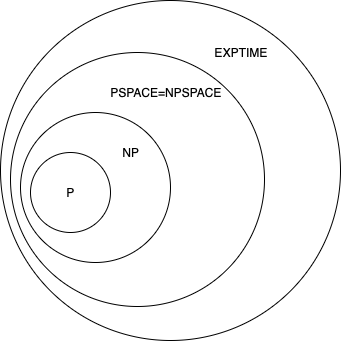
\includegraphics[scale=0.6]{NP-PSPACE}
\end{figure}
\subsubsection{PSPACE-completezza}
Un linguaggio B è PSPACE-completo se soddisfa due condizioni:
\begin{enumerate}
	\item $B \in PSPACE$
	\item $\forall \text{A in PSPACE, }A \leq_{p} B$
\end{enumerate}
Notare che è necessario effettuare la riduzione in tempo polinomiale e non in spazio polinomiale, questo perché una macchina che usa spazio polinomiale può impiegare $2^{O(n^k)}$.
\subsection{Esercizi}
1. $L \in NSPACE(n^2)$, per quale $f(n) \ L \in TIME(f(n))$

Usando il teorema Savitch, abbiamo che:
\[
	L \in NSPACE(n^2) \Rightarrow L \in SPACE(n^4) \Rightarrow TIME(2^{O(n^4)})
\]

Non usando il teorema Savitch, devo passare da NTM a TM usando la costruzione

con l'albero, quindi $L \in TIME(2^{2^{O(n^2)}})$.
\\

Bisogna controllare quale costruzione da NTM a TM restituisce il risultato migliore.
\\
2. $L \in NTIME(n^2)$, per quale $f(n) \ L \in SPACE(f(n))$

Usando il teorema di Savitch abbiamo che:


Sapendo che il tempo limita lo spazio $L \in NTIME(n^2) \Rightarrow L \in NSPACE(n^2)$, quindi:

\[
	L \in NTIME(n^2) \Rightarrow L \in NSPACE(n^2) \Rightarrow L \in SPACE(n^4)
\]

Non usando il teorema di Savitch vedo quanto spazio occupano i nastri:

\[
\left.
\begin{aligned}
&\text{nastro di input O(n)}\\
&\text{nastro di lavoro $O(n^2)$}\\
&\text{nastro guida $O(n^2)$}
\end{aligned}
\right\rbrace
\text{$\Rightarrow L \in SPACE(n^2)$}
\]

Se si parte da NTIME è consigliato usare la costruzione tramite l'albero, se si parte da 

NSPACE invece è consigliato usare il teorema di Savitch
\\
3. $A \leq_{m} \overline{A} \ A \in Turing-Riconoscibile$, cosa posso dire di $\overline{A}$

\[
	A \leq_{m} \overline{A} \Rightarrow \overline{A} \leq_{m} A \Rightarrow \overline{A} \in Turing-Riconoscibile
\]
4. $SAT \in SPACE(n) \rightarrow SAT \in TIME(2^{O(n)}$
\subsection{Algoritmo $ALL_{NFA}$}
$ALL_{NFA} = \{ <A> \ \mid A \in NFA_{\Sigma} \text{ e } L(A)=\Sigma^{\star} \}$
\\
$\overline{ALL_{NFA}} = \{ <A> \ \mid A \in NFA_{\Sigma} \text{ e } L(A) \neq \Sigma^{\star} \}$
\\\\
M: input $<A>, \ A \in NFA_{\Sigma}$

output: si se $L(A) \neq \Sigma^{\star}$

\quad \quad \quad \ \ no altrimenti
%VI PREGO RISOLVETE QUESTO SCHIFO CHE NON SONO RIUSCITO A TROVARE QUALCOSA PER FARE DI MEGLIO!!!!!!!
\begin{enumerate}
	\item $S = \varepsilon-closure$
	\item Ripeti $2^q$ volte, dove $q=|Q|$ di A (q è il massimo numero di stati della macchina deterministica di A che simula la macchina non deterministica di A)
	\begin{enumerate}[label*=\arabic*.]
		\item se S non contiene uno stato finale, accetta
		\item non deterministicamente prendi $a \in \Sigma$ e calcola $S' = \varepsilon-closure ( \bigcup_{p \in S} \delta (p,a) )$
		\item poni $S = S'$ (e ricomincia)
	\end{enumerate}
\end{enumerate}
Il più grande insieme S che considero ha q elementi, e occupa spazio O(n), dove n è la lunghezza della codifica di A: $n=|<A>| \quad n \geq q$
\\\\
$\overline{ALL_{NFA}} \in NSPACE(n)$ \newpage